%%%%%%%%%%%%%%%%%%%%%%%%%%%%%%%%%%%%%%%%%%%%%%%%%%%%%%%%%%%%%%%%%%%%%
%% sec_benchmarks.tex
%% Section 4: Numerical Results
%% RMG Periodic RT-TDDFT — Paper 2
%%
%% All four benchmark figures are in paper2/Figs/:
%%   out-h2.pdf   -- H2 chain (1D)
%%   out-hBN.pdf  -- hexagonal BN (2D)
%%   out-Si.pdf   -- Si crystal (3D)
%%   out-CrI3.pdf -- CrI3 (spin-polarized)
%%%%%%%%%%%%%%%%%%%%%%%%%%%%%%%%%%%%%%%%%%%%%%%%%%%%%%%%%%%%%%%%%%%%%

\section{Numerical Results}
\label{sec:results}

We benchmark the periodic and spin-polarized RT-TDDFT implementation
in \texttt{RMG} against the \texttt{Octopus} code\cite{octopus} for
four representative systems of increasing dimensionality and physical
complexity: a one-dimensional hydrogen chain (H$_2$), a
two-dimensional hexagonal boron nitride (hBN) monolayer, a
three-dimensional silicon crystal, and the spin-polarized magnetic
insulator \ch{CrI3}.
These systems are chosen to isolate and validate specific aspects of
the implementation: k-point sampling, anisotropic optical response,
three-dimensional periodic boundaries, and spin-collinear propagation,
respectively.
The section concludes with a demonstration of the unique large-scale
capability of \texttt{RMG} through calculations on nitrogen-vacancy
(NV) centers in diamond at varying supercell sizes.

In all calculations, a momentum kick of amplitude $E_0 =
\myblue{[\mathrm{value}]}$~a.u.\ was applied at $t=0$ along each
Cartesian direction independently, and the optical conductivity
was obtained from the Fourier transform of the resulting current
density.
\myblue{[Add: common computational parameters -- time step, total
propagation time, broadening gamma, XC functional, pseudopotential
library used for all systems.]}

%--------------------------------------------------------------------
\subsection{One-Dimensional Periodic System: Hydrogen Chain}
\label{sec:h2}
%--------------------------------------------------------------------

As the simplest possible periodic test system, we consider an
infinite chain of hydrogen molecules aligned along the $z$ axis
with alternating bond lengths, modeled by a one-dimensional
supercell with periodic boundary conditions.
This system provides a stringent test of k-point sampling and the
velocity gauge implementation in the limit of a quasi-one-dimensional
geometry, where the longitudinal ($z$-direction) and transverse
($x$, $y$-direction) optical responses differ substantially.

\myblue{[Computational details:
- Supercell geometry: H--H bond length, H$_2$--H$_2$ separation
- K-point sampling: \myblue{[N\_k points along z, Gamma in x and y]}
- Grid spacing: \myblue{[value]} a$_0$
- XC functional: \myblue{[PBE or LDA]}
- Pseudopotential: \myblue{[type]}
- Time step $\Delta t$: \myblue{[value]} a.u.
- Total simulation time: \myblue{[value]} a.u.
- Broadening $\gamma$: \myblue{[value]} eV]}

\begin{figure}[ht!]
  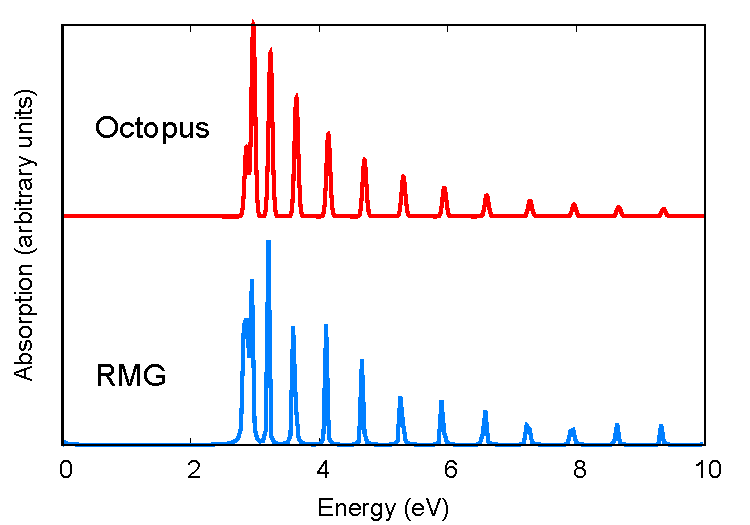
\includegraphics[width=\columnwidth]{Figs/out-h2.pdf}
  \caption{\footnotesize
    \myblue{[Caption for H$_2$ chain optical conductivity figure.
    Should describe: (a) longitudinal $\sigma_{zz}(\omega)$ and
    transverse $\sigma_{xx}(\omega)$ components from RMG compared
    with Octopus; (b) convergence with k-point density if shown;
    labels for RMG and Octopus curves.
    Note anisotropy of 1D system as key feature to highlight.]}
  }
  \label{fig:h2}
\end{figure}

\myblue{[Discussion points:
- Agreement between RMG and Octopus for both longitudinal and
  transverse components
- K-point convergence: how many k-points needed for converged spectrum?
- Physical interpretation of the spectral features
- If Berry phase comparison is available: show agreement between
  current-integration and BP polarization as internal consistency check
  (Fruit 1 from CONTEXT.md)
- If ground-state current convergence is shown: include as panel or
  note in text (Fruit 2 from CONTEXT.md)]}


%--------------------------------------------------------------------
\subsection{Two-Dimensional Periodic System: Hexagonal Boron Nitride}
\label{sec:hbn}
%--------------------------------------------------------------------

Hexagonal boron nitride (hBN) is a wide-gap insulating two-dimensional
material with $D_{6h}$ symmetry.
Its optical response is highly anisotropic: the in-plane conductivity
$\sigma_{xx}(\omega) = \sigma_{yy}(\omega)$ differs markedly from the
out-of-plane component $\sigma_{zz}(\omega)$, the latter being
negligible for photon energies below the interlayer excitations.
This system tests the implementation of two-dimensional periodic
boundary conditions and the symmetry enforcement of the conductivity
tensor in \texttt{RMG}.

\myblue{[Computational details:
- Monolayer geometry: lattice constant \myblue{[a]} \AA,
  vacuum layer \myblue{[d]} \AA\ to prevent inter-layer interactions
- K-point sampling: \myblue{[N\_k $\times$ N\_k $\times$ 1]} Monkhorst-Pack
- Grid spacing: \myblue{[value]} a$_0$
- XC functional: \myblue{[PBE]}
- Pseudopotential: \myblue{[type]}
- Time step and total simulation time: \myblue{[values]}]}

\begin{figure}[ht!]
  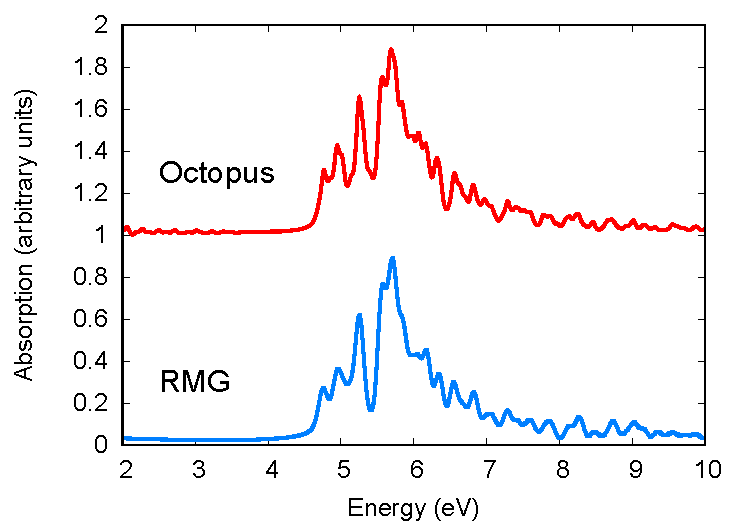
\includegraphics[width=\columnwidth]{Figs/out-hBN.pdf}
  \caption{\footnotesize
    \myblue{[Caption for hBN optical conductivity figure.
    Should describe: in-plane $\sigma_{xx}(\omega)$ from RMG and
    Octopus; out-of-plane component if shown; indicate the onset
    of absorption near the band gap.
    Highlight that $\sigma_{xx}=\sigma_{yy}$ (symmetry correctly
    reproduced) and $\sigma_{zz}\approx 0$.]}
  }
  \label{fig:hbn}
\end{figure}

\myblue{[Discussion points:
- Agreement between RMG and Octopus for in-plane conductivity
- Symmetry: show that $\sigma_{xx}=\sigma_{yy}$ (Fruit 3 from CONTEXT.md)
- Physical features: onset at band gap, first excitonic peak if visible
- Comparison with available experimental or LR-TDDFT data if relevant]}


%--------------------------------------------------------------------
\subsection{Three-Dimensional Periodic System: Silicon}
\label{sec:si}
%--------------------------------------------------------------------

Silicon in the diamond cubic structure ($F d\bar{3}m$, space group 227)
is the canonical benchmark for periodic electronic structure
calculations.
Its indirect band gap and well-characterized optical spectrum provide
a rigorous test of the full three-dimensional periodic RT-TDDFT
implementation.
The cubic symmetry requires $\sigma_{xx}(\omega) = \sigma_{yy}(\omega)
= \sigma_{zz}(\omega)$, providing an immediate symmetry validation.

\myblue{[Computational details:
- Unit cell: conventional 8-atom cell, lattice constant \myblue{[a]} \AA
- K-point sampling: \myblue{[N\_k $\times$ N\_k $\times$ N\_k]} Monkhorst-Pack
- Grid spacing: \myblue{[value]} a$_0$
- XC functional: \myblue{[PBE]}
- Pseudopotential: \myblue{[type, NCPP]}
- Number of occupied + virtual states: \myblue{[N\_occ + N\_virt]}
- Time step $\Delta t$: \myblue{[value]} a.u.
- Total simulation time: \myblue{[value]} a.u. (\myblue{[value]} fs)
- Broadening $\gamma$: \myblue{[value]} eV]}

\begin{figure}[ht!]
  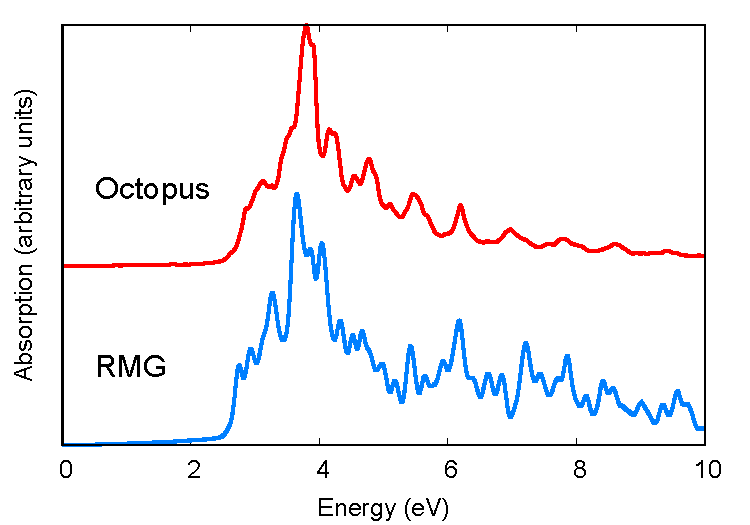
\includegraphics[width=\columnwidth]{Figs/out-Si.pdf}
  \caption{\footnotesize
    \myblue{[Caption for Si optical conductivity figure.
    Should describe: $\sigma_{xx}(\omega)$ (= $\sigma_{yy}$ = $\sigma_{zz}$
    by cubic symmetry) from RMG compared with Octopus;
    indicate band gap region; optionally compare with experiment.
    If energy conservation panel included: describe it.]}
  }
  \label{fig:si}
\end{figure}

\myblue{[Discussion points:
- Agreement between RMG and Octopus: peak positions, lineshapes
- Symmetry: $\sigma_{xx}=\sigma_{yy}=\sigma_{zz}$ (Fruit 3)
- Energy conservation test for periodic case (Fruit 5 from CONTEXT.md):
  run longer simulation and show no drift, analogous to paper 1 Fig.~3c
- Berry phase comparison if included (Fruit 1)
- Physical features: onset near direct gap, main optical peak structure]}


%--------------------------------------------------------------------
\subsection{Spin-Polarized System: \ch{CrI3}}
\label{sec:cri3}
%--------------------------------------------------------------------

Chromium triiodide (\ch{CrI3}) is a layered van der Waals magnetic
insulator with a honeycomb lattice of \ch{Cr^{3+}} ions, each carrying
a local moment of approximately $3\,\mu_B$.
In its ferromagnetic ground state, the spin-up and spin-down electronic
structures differ, leading to distinct optical spectra for the two
spin channels.
This system provides a direct test of the spin-collinear RT-TDDFT
extension: the two spin channels should propagate independently but
with a common Hartree potential, yielding spin-resolved optical
conductivities that can be compared with \texttt{Octopus} and with
available experimental data.

\myblue{[Computational details:
- Unit cell: \myblue{[describe geometry and magnetic ordering]}
- K-point sampling: \myblue{[N\_k $\times$ N\_k $\times$ N\_k]}
- XC functional: \myblue{[PBE or PBE+U; specify U if used]}
- Pseudopotential: \myblue{[type, NCPP]}
- Initial spin configuration: ferromagnetic, moments on Cr sites
- Time step and total simulation time: \myblue{[values]}
- Broadening: \myblue{[value]} eV]}

\begin{figure}[ht!]
  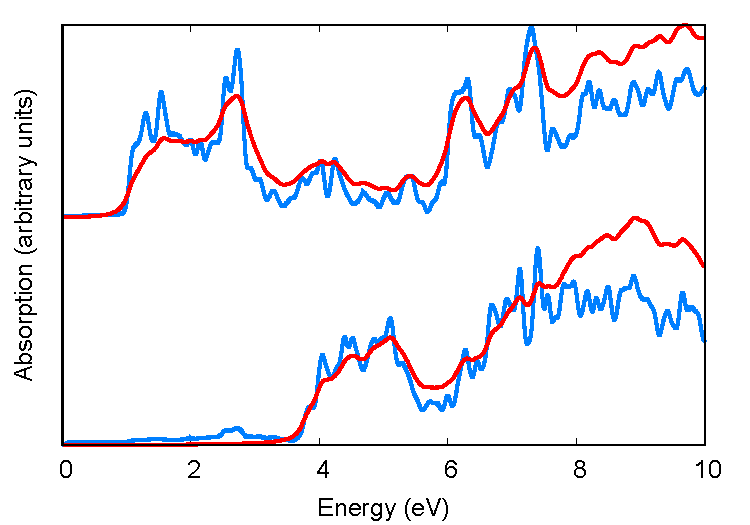
\includegraphics[width=\columnwidth]{Figs/out-CrI3.pdf}
  \caption{\footnotesize
    \myblue{[Caption for \ch{CrI3} optical conductivity figure.
    Should describe: spin-up and spin-down optical conductivities
    from RMG compared with Octopus; indicate the relevant spectral
    features (charge-transfer peaks, d-d transitions);
    note that spin channels are labeled consistently.]}
  }
  \label{fig:cri3}
\end{figure}

\myblue{[Discussion points:
- Agreement between RMG and Octopus for both spin channels
- Physical interpretation: which spectral features are spin-up vs spin-down?
  Charge-transfer excitations, Cr d-d transitions
- Spin current $\mathbf{J}_{\mathrm{spin}} = \mathbf{J}^\uparrow
  - \mathbf{J}^\downarrow$ if computed (Fruit 4 from CONTEXT.md)
- Comparison with available experimental optical data if relevant
- Note: ECD/MCD spectra not computed in this work (magnetic perturbation
  formalism reserved for future publication)]}


%--------------------------------------------------------------------
\subsection{Large-Scale Demonstration: NV Center in Diamond}
\label{sec:nv}
%--------------------------------------------------------------------

As a final demonstration, we apply the periodic spin-polarized RT-TDDFT
implementation to the negatively charged nitrogen-vacancy (NV$^-$)
center in diamond, one of the most studied point defects in
solid-state physics.\cite{NV-Doherty-2013,NV-Gali-2008,NV-Gali-2019,nv-center-review}
This system tests several capabilities simultaneously: spin-polarized
real-time propagation, the optical response of a localized defect in a
three-dimensional periodic host, convergence toward the dilute-defect
limit, and computational scaling to thousands of atoms.

The NV$^-$ center consists of a substitutional nitrogen atom adjacent
to a carbon vacancy, oriented along a $\langle111\rangle$
crystallographic direction, with one additional trapped electron. Its
ground state is an optically addressable spin triplet, with defect
molecular orbitals located within the diamond band
gap.\cite{NV-Gali-2008,NV-Gali-2019,NV-Louie-2012} Its long spin
coherence time at room temperature makes it central to nanoscale
magnetometry, quantum sensing, single-photon emission, and quantum
information processing.\cite{NV-coherence-Balasubramanian-2009,NV-sensing-Degen-2017,NV-sensing-Maze-2008,NV-sensing-Schirhagl-2014,NV-spe-Aharonovich-2016,NV-QComp-Bradley-2019}

In a standard periodic DFT or RT-TDDFT calculation the NV$^-$ center is
represented by a single defect in a periodically repeated supercell.
The physical properties of the \emph{isolated} defect are recovered
only once the supercell is large enough that the interaction between
the defect and its periodic images is negligible; identifying this
convergence threshold is both a practical necessity and a physically
meaningful result, since it establishes the minimum defect
concentration at which the isolated-defect limit is reached.

The purpose of our demonstration is not to provide a complete
many-body description of the NV$^-$ photophysics, which involves
vibronic effects, singlet-triplet manifolds, and charge-state physics,
but to demonstrate large-scale spin-polarized real-time simulations of
optical response for increasing supercell size and defect
concentration.

\subsubsection{Electronic Structure and Optical Selection Rule}
\label{sec:nv-electronic-structure}

The NV$^-$ triplet ground state ($^3A_2$) has the single-particle
configuration $a_1^2 e^1 e^1$: a doubly-occupied, non-degenerate $a_1$
orbital located primarily on the nitrogen atom with contributions from
the three neighboring carbon atoms, and two singly-occupied, degenerate
$e$-symmetry orbitals formed from those same three carbons. Both $a_1$
and $e$ lie within the diamond band gap. Under the $C_{3v}$ point group
of the defect, the two-electron product decomposes as
$E\times E = A_1 + A_2 + E$, so the lowest excited configuration
obtained by promoting one electron from $a_1$ into $e$ is itself
doubly degenerate, matching the well-known $^3E$ excited state.
Concretely, the two microstates spanning the $^3E$ manifold correspond
to promoting the minority-spin ($\downarrow$) electron out of $a_1$
into either of the two degenerate $e$ orbitals; the resulting
$^3A_2\rightarrow{}^3E$ transition is the origin of the well-known
zero-phonon line (ZPL) at $1.94$~eV.\cite{NV-Gali-2008,NV-Gali-2019}

Because $E$ transforms as the in-plane representation $(x,y)$ under
$C_{3v}$ (with the $C_3$ axis along the defect's $\langle111\rangle$
axis), the $^3A_2\rightarrow{}^3E$ transition dipole is confined to the
plane perpendicular to $\langle111\rangle$: it is symmetry-forbidden
for light polarized along $\langle111\rangle$ and allowed for any
polarization within the perpendicular plane. We tested this directly
by applying the RT-TDDFT delta-kick perturbation along three
directions: $[111]$ (parallel to $C_3$), and $[1\bar{1}0]$ and
$[11\bar{2}]$ (both perpendicular to $C_3$). The ZPL feature is absent
for the $[111]$ kick and present, at essentially the same strength,
for both perpendicular directions, with the residual signal along
$[111]$ smaller by roughly a factor of $50$---consistent with, and
substantially exceeding, the group-theory prediction. The ZPL feature
further appears predominantly in the spin-down channel, exactly as
expected from the $a_1(\downarrow)\rightarrow e(\downarrow)$ assignment
above: the spin-up manifold has no corresponding low-lying transition
available at this energy, since both spin-up $e$ orbitals are already
singly occupied in the ground state.
\myblue{[Figure placeholder: three-panel polarization comparison,
$[111]$ vs.\ $[1\bar{1}0]$ vs.\ $[11\bar{2}]$, spin-up/spin-down
resolved. Correct the axis-label parallel/perpendicular assignment
before finalizing the source figure---the underlying data are
correct, only the descriptive labels need fixing.]}

This result is independent of the supercell-size and active-space
convergence questions addressed below: it follows from the defect's
point-group symmetry alone, and therefore validates the
implementation's velocity-gauge, polarization-resolved response
independently of any of the numerical convergence caveats that follow.
\myblue{[Optional: brief note/plots of the $a_1$ and $e$ defect-orbital
isosurfaces and/or spin density, if included.]}

\subsubsection{Linear-Response Optics (LOPTICS): An Independent Ground-State Cross-Check}
\label{sec:nv-loptics}

Throughout the remainder of this demonstration we cross-validate our
RT-TDDFT spectra against RMG's ground-state linear-response optics
module (\texttt{LOPTICS}), which evaluates the imaginary part of the
dielectric tensor directly from a sum over Kohn-Sham states, with no
time propagation involved. In atomic units,
\begin{equation}
  \epsop_2^{\alpha\beta}(\omega) =
  \frac{4\pi^2}{\Omega\,\omega^2}
  \sum_{\mathbf{k}} w_{\mathbf{k}}
  \sum_{v,c}
  \left(f_{v\mathbf{k}} - f_{c\mathbf{k}}\right)
  \Jmat{\alpha}_{vc}(\mathbf{k})\,
  \left[\Jmat{\beta}_{vc}(\mathbf{k})\right]^{*}
  \,\delta\!\left(E_{c\mathbf{k}} - E_{v\mathbf{k}} - \hbar\omega\right),
  \label{eq:loptics}
\end{equation}
where $\Omega$ is the unit-cell volume, $w_{\mathbf{k}}$ the k-point
weight, $f_{n\mathbf{k}}$ the occupation of state $n$ at $\mathbf{k}$,
and the sum runs over occupied ($v$) and unoccupied ($c$) Kohn-Sham
states. The real part $\epsop_1(\omega)$ is reconstructed afterward via
a Kramers-Kronig transform, and the energy-conserving $\delta$-function
is represented numerically by a Gaussian, re-broadened with a
Lorentzian whose width sets the effective spectral resolution.

Critically, the matrix element $\Jmat{\alpha}_{vc}(\mathbf{k})$ entering
Eq.~\eqref{eq:loptics} is \emph{identical} to the current-operator
matrix element defined in Eq.~\eqref{eq:Jmat-full}
(Sec.~\ref{sec:current-dm-sec}) and used throughout the real-time
propagation: it includes the same nonlocal-pseudopotential correction,
computed by the same underlying routine, not a bare momentum matrix
element. LOPTICS and RT-TDDFT therefore start from exactly the same
physical ingredients---ground-state Kohn-Sham orbitals and the same
gauge-consistent current operator---and differ only in how the optical
response is extracted from them: LOPTICS by direct sum-over-states
evaluation in the frequency domain, RT-TDDFT by explicit real-time
propagation followed by a Fourier transform. Because LOPTICS's
frequency resolution is set only by the chosen broadening, rather than
by a finite propagation time, it provides an essentially exact
reference against which the resolution-limited real-time spectra can be
validated, as used throughout the rest of this section. No local-field
correction is included at this level, consistent with an
independent-particle treatment of the response.

\subsubsection{Convergence with Supercell Size and Brillouin-Zone Sampling}
\label{sec:nv-convergence}

We investigate the approach to the isolated-defect limit using a
matrix of diamond supercells spanning three sizes and, for the two
smaller sizes, two Brillouin-zone samplings each: a $64$-atom
supercell at both $\Gamma$ and a $4\times4\times4$ Monkhorst-Pack mesh;
a $512$-atom supercell at both $\Gamma$ and a $2\times2\times2$ mesh;
and a $4096$-atom supercell at $\Gamma$ only, each containing a single
NV$^-$ center.

\begin{table}[ht]
\centering
\begin{tabular}{lll}
\hline
System & $k$-mesh & Result \\
\hline
$64$ atoms  & $\Gamma$ & single dominant peak, $\sim\!1.9$~eV \\
$64$ atoms  & $4\times4\times4$ & multiplet, $\sim\!1.4$--$2.4$~eV \\
$512$ atoms & $\Gamma$ & single peak, $\sim\!1.93$~eV \\
$512$ atoms & $2\times2\times2$ & \myblue{[RT-TDDFT currently shows a
  single peak at short propagation time; re-running at longer
  propagation to test whether the LOPTICS-predicted splitting (below)
  is a genuine feature or a resolution artifact of the shorter
  run---insert final result]} \\
$4096$ atoms & $\Gamma$ & single dominant peak; position depends on
  active-space size (Sec.~\ref{sec:nv-active-space}) \\
\hline
\end{tabular}
\caption{\footnotesize Summary of the supercell-size/$k$-sampling test
matrix. RT-TDDFT results are cross-validated by LOPTICS
(Sec.~\ref{sec:nv-loptics}) at every entry; agreement is close except
where noted.}
\label{tab:nv-matrix}
\end{table}

At fixed cell size, it is moving from $\Gamma$-only to a dense $k$-mesh
that reveals the multiplet structure at $64$ atoms, not the reverse.
This is an important point for interpreting the table: a clean,
single-peak spectrum obtained at $\Gamma$ in a small cell is
\emph{not}, by itself, evidence that the defect is behaving as an
isolated emitter---it only means that a single point of what may still
be a dispersive, defect-coupled band has been sampled. Only when the
spectrum becomes insensitive to $k$-sampling, as it does between $64$
and $512$ atoms, can convergence toward the isolated-defect limit be
claimed with confidence. By this criterion, LOPTICS indicates that
even the $512$-atom cell has not fully reached that limit: at
$2\times2\times2$ sampling it resolves a split peak that is not visible
in the $\Gamma$-only result at the same size, implying non-negligible
residual defect-image coupling even at $512$ atoms.
\myblue{[State the resolution once the longer RT-TDDFT run at $512$
atoms/$2\times2\times2$ completes: either (a) RT-TDDFT recovers the
same splitting once propagated long enough, confirming the coupling is
real and that the earlier single-peak appearance was a
finite-propagation-time resolution artifact, or (b) the methods
genuinely disagree, which would need further investigation.]}

An equivalent, and computationally more natural, way to probe the
$512$-atom/$2\times2\times2$ result is via the real-space
supercell-folding equivalence: a $k\times k\times k$ Monkhorst-Pack
sampling of a cell is formally equivalent to a $\Gamma$-only
calculation on the $k^3$-fold real-space replica of that cell, provided
the replica's self-consistent solution respects the same periodicity as
the original cell (i.e., no explicit symmetry-breaking to a larger
magnetic unit cell). The $2\times2\times2$ real-space replica of the
$512$-atom cell is precisely the $8$-defect, $4096$-atom system used in
Sec.~\ref{sec:nv-fm-afm} below; propagating that system at $\Gamma$
only, in its translationally-simple (ferromagnetic) configuration,
provides a second, independent route to the same
$512$-atom/$2\times2\times2$ answer, without the added cost and
complexity of explicit non-$\Gamma$ real-time propagation.
\myblue{[Confirm numerically that the $\Gamma$-only, FM-configuration
result for the $8$-defect/$4096$-atom system matches the direct
$512$-atom/$2\times2\times2$ result, as the folding argument predicts.]}

\myblue{[Computational details:
- Host: diamond cubic, lattice constant \myblue{[a]}~\AA
- Defect: single NV$^-$ center (negatively charged)
- Spin state: triplet ground state ($S=1$)
- XC functional: \myblue{[value]}; Pseudopotential: \myblue{[value]}
- Active space (production, total states): $64$ atoms:
  $N_{\mathrm{basis}}=13{,}640$ ($\approx\!213$/atom); $512$ atoms:
  $N_{\mathrm{basis}}=13{,}696$ ($\approx\!27$/atom); $4096$ atoms:
  $N_{\mathrm{basis}}=13{,}696$ ($\approx\!3.3$/atom)---see
  Sec.~\ref{sec:nv-active-space} for the convergence implications of
  this shrinking per-atom ratio
- Time step and total propagation time: \myblue{[values]}
- Computational platform: Frontier at ORNL; nodes used:
  \myblue{[values per system size]}]}

\begin{figure}[ht!]
  \myblue{[Figure: RT-TDDFT and LOPTICS spectra overlaid for each row
  of Table~\ref{tab:nv-matrix}, on a common energy axis. Label the ZPL
  region and, for the $64$-atom/$4\times4\times4$ case, the multiplet
  envelope.]}
  \caption{\footnotesize \myblue{[Caption describing the convergence
  behavior and identifying the minimum supercell size at which the
  isolated-defect spectrum is recovered, per the $k$-sensitivity
  criterion above.]}}
  \label{fig:nv}
\end{figure}

\subsubsection{Active-Space Convergence: Virtual Orbitals and the Occupied-State Window}
\label{sec:nv-active-space}

Reaching the $4096$-atom system size requires reducing the active
space---the set of Kohn-Sham states actually propagated in real
time---well below what is used for the smaller systems, purely for
computational cost. Two independent truncations are available: the
number of virtual (initially unoccupied) states added above the
physically occupied manifold (the RMG input key
\texttt{unoccupied\_states\_per\_kpoint}, denoted $N_{\mathrm{virt}}$
below---not $N_{\mathrm{occ}}$ as in our working notes, since it is the
virtual-state count that is varied), and the index of the lowest
occupied state included in the propagation
(\texttt{tddft\_start\_state}), below which states are frozen at fixed
occupation and do not contribute to the time-dependent density. The
total active-space size achievable within a fixed compute budget is
comparable across system sizes ($N_{\mathrm{basis}}\approx13{,}600$--
$13{,}700$ states, Sec.~\ref{sec:nv-convergence}), so the resulting
per-atom active space falls sharply with system size: roughly $213$
states/atom at $64$ atoms, $27$ states/atom at $512$ atoms, and only
$3.3$ states/atom at $4096$ atoms.

Independently varying \texttt{tddft\_start\_state} at fixed
$N_{\mathrm{virt}}$, and $N_{\mathrm{virt}}$ at fixed occupied window,
at $512$ atoms shows that both truncations shift the computed ZPL, with
the virtual-side truncation producing the larger effect. Truncating the
occupied window at fixed $N_{\mathrm{virt}}=3200$ moves the peak from
$\approx\!1.93$~eV at \texttt{tddft\_start\_state}$=0$---in close
agreement with the experimental value of $1.94$~eV---to
$\approx\!2.05$~eV at \texttt{tddft\_start\_state}$=800$ (of $1024$
valence states); the corresponding $N_{\mathrm{virt}}$ sweep at fixed
occupied window produces a substantially larger shift over a comparable
range of active-space reduction. Both trends are the expected signature
of a variationally under-converged excited state, not a numerical
artifact: in the linear-response regime, RT-TDDFT is equivalent to the
poles of the same response function obtained from a Casida-type
eigenvalue problem in the same active space, and enlarging a
\emph{nested} particle-hole excitation space---exactly what increasing
$N_{\mathrm{virt}}$ or decreasing \texttt{tddft\_start\_state}
does---can only improve, never worsen, each ordered approximate root (a
Hylleraas--Undheim/MacDonald-type interlacing result, the same
principle behind the monotonic improvement of a truncated-CI
excited-state energy with basis size). The same direction of shift is
seen at $4096$ atoms across active-space settings spanning
$N_{\mathrm{virt}}=4000$--$9000$, confirming the trend persists at the
flagship system size.

The production active-space sizes used for the size-convergence results
in Sec.~\ref{sec:nv-convergence} are $N_{\mathrm{basis}}=13{,}640$,
$13{,}696$, and $13{,}696$ for the $64$-, $512$-, and $4096$-atom
systems respectively---a comparable total active-space size across all
three, rather than a fixed per-atom ratio, reflecting the largest
active space practically feasible within a common compute budget at
each size.
\myblue{[Report the resulting ZPL peak position at these final
production settings for each system size, superseding the exploratory
values quoted above for illustrating the convergence trend.]}

Because the resulting per-atom active space is far smaller at $4096$
atoms ($3.3$ states/atom) than at $512$ atoms ($27$ states/atom), the
larger deviation of the flagship system's peak position from the
experimental ZPL is most plausibly dominated by active-space
truncation rather than by residual defect-image coupling---the latter
having already been shown, in Sec.~\ref{sec:nv-convergence}, to become
small well before $4096$ atoms. This mirrors the active-space
convergence study already performed for finite systems in paper 1
(benzene, C$_{60}$, and Ag nanorods), extended here to a periodic
defect with an additional, occupied-side truncation knob that the
finite-system case did not require. Sec.~\ref{sec:nv-fm-afm} below
provides a direct, controlled test of this attribution: by comparing
the $1$-, $8$-, and $64$-defect systems at the \emph{same} total size,
and therefore the \emph{same} $N_{\mathrm{virt}}$, any peak-position
difference between them isolates the concentration/defect-image-coupling
effect specifically, with active-space truncation held fixed as a
common systematic across all three.
\myblue{[Figure placeholder: peak position vs.\ $N_{\mathrm{virt}}$ (at
$512$ and $4096$ atoms) and vs.\ \texttt{tddft\_start\_state} (at
$512$ atoms), showing the monotonic approach toward the experimental
ZPL.]}
\myblue{[If feasible, report an extrapolated or higher-$N_{\mathrm{virt}}$
result for the $4096$-atom system, using the $512$-atom active-space
sweep as a calibration for the expected remaining shift.]}

\subsubsection{Concentration-Matched Comparison: Ferromagnetic versus Antiferromagnetic Defect Ordering}
\label{sec:nv-fm-afm}

The supercell-size convergence study above varies defect concentration
and total simulation-cell size together: each cell contains exactly one
NV center, so lowering the defect density is only possible by enlarging
the cell. To isolate the effect of defect concentration from that of
absolute cell size, we make further use of the $8$-defect,
$4096$-atom replica introduced in Sec.~\ref{sec:nv-convergence}, and
construct one additional, more concentrated companion system: a
$4\times4\times4$ real-space replica of the $64$-atom (single-defect)
cell, yielding $64$ NV centers in a $4096$-atom host. Together with the
original single-defect $4096$-atom calculation, these three
systems---$64$, $8$, and $1$ NV centers---share an identical
simulation-cell size and real-space grid, differing only in defect
concentration, by two orders of magnitude. Crucially, because all three
share the same total atom count, they can also be propagated with the
\emph{same} active-space size $N_{\mathrm{virt}}$---unlike the direct
single-defect size series in Sec.~\ref{sec:nv-convergence}, where
$N_{\mathrm{virt}}$ per atom necessarily shrinks as the cell grows.
This is a deliberate design choice rather than an incidental
convenience: it allows any peak-position shift among the $1$-, $8$-,
and $64$-defect results to be attributed to defect concentration
specifically, rather than to the confound between active-space
truncation and system size identified in
Sec.~\ref{sec:nv-active-space}. All three systems use
$N_{\mathrm{virt}}=8200$ ($\approx\!2$ virtual orbitals per carbon
atom) and \texttt{tddft\_start\_state}$=2700$, a deliberate compromise
between the two $4096$-atom active-space choices discussed in
Sec.~\ref{sec:nv-active-space}: closer to full occupancy than the
$N_{\mathrm{virt}}=9000$/\texttt{tddft\_start\_state}$=4100$ setting,
but with a substantially larger virtual space than the initial
$N_{\mathrm{virt}}\approx\!4000$/\texttt{tddft\_start\_state}$=0$
setting.
\myblue{[Confirm: is the $1$-defect entry in this comparison a fresh
calculation at these compromise settings, or is it identical to one of
the two $4096$-atom results already reported in
Sec.~\ref{sec:nv-active-space}? If the former, the two should be
distinguished explicitly rather than both called ``the $4096$-atom
single-defect result.'']}

At these densities the individual $S=1$ spin-triplet defect moments are
no longer independent, and the relevant physical question becomes how
they order relative to one another. We consider two limiting
configurations: a ferromagnetic (FM) arrangement, in which all defect
spins are aligned parallel, and an antiferromagnetic (AFM) arrangement,
in which neighboring defect moments alternate in sign across the defect
lattice. The total-energy difference between these two configurations,
\begin{equation}
  \Delta E_{\mathrm{FM-AFM}} = E_{\mathrm{FM}} - E_{\mathrm{AFM}},
\end{equation}
provides an estimate of the effective magnetic exchange coupling between
NV centers mediated through the diamond host, analogous to exchange
constants extracted from broken-symmetry DFT calculations of
multi-radical or polynuclear transition-metal
systems.\myblue{[cite: broken-symmetry / Heisenberg exchange reference]}

Preliminarily, we find the ferromagnetic configuration to be
energetically favored over the antiferromagnetic configuration
\emph{at both defect concentrations} (8- and 64-defect systems), with
$\Delta E_{\mathrm{FM-AFM}} = \myblue{[\text{value, meV or meV/defect}]}$
for the $64$-defect system and
$\myblue{[\text{value}]}$ for the $8$-defect system.
\myblue{[Comment on whether the coupling strengthens or weakens with
increasing defect separation (i.e.\ between the $64$- and $8$-defect
cases), consistent with a superexchange- or wavefunction-overlap-mediated
mechanism rather than long-range dipolar coupling.]}

We have additionally computed the linear optical response (LOPTICS, see
Sec.~\ref{sec:nv-loptics}) for both the FM and AFM configurations at both
defect concentrations, providing a converged baseline against which the
corresponding real-time spectra can be validated once available.
\myblue{[Figure placeholder: LOPTICS spectra for FM vs.\ AFM
configurations, $64$- and $8$-defect systems, compared against the
single-defect ($1$-defect) $4096$-atom reference spectrum from
Fig.~\ref{fig:nv}. Discuss whether magnetic ordering produces a
resolvable spectral signature, or whether the FM and AFM optical
responses are nearly indistinguishable at these concentrations.]}
\myblue{[RT-TDDFT real-time spectra for the FM and AFM systems: still
running at time of writing---insert once complete, using the LOPTICS
results above as the reference for judging active-space and
propagation-length convergence.]}

We note that we have not performed an analogous
$\Gamma$-versus-$2\times2\times2$ LOPTICS check on the single-defect
$4096$-atom reference system used as the $1$-defect baseline above.
\myblue{[State explicitly: based on the trend established in the main
convergence study (defect-image coupling decreasing monotonically with
cell size/increasing real-space defect separation), we do not expect
qualitative changes at this size; a dense-k check is left for future
work, e.g.\ in response to reviewer request.]}

This comparison illustrates a further capability unique to a
massively-scalable real-time implementation: beyond recovering the
isolated-defect limit for a single center, RMG can directly address
ensembles of interacting quantum defects at densities relevant to real
NV-diamond samples, opening a path toward studying emergent collective
phenomena---magnetic ordering and defect-defect optical
coupling---that are inaccessible to small-cell approaches.
%%%%%%%%%%%%%%%%%%%%%%%%%%%%%%%%%%%%%%
\section{ OpenAI}
%--------------------------------------------------------------------
\subsection{Large-Scale Demonstration: NV$^-$ Center in Diamond}
\label{sec:nv}
%--------------------------------------------------------------------

As a final demonstration, we apply the periodic spin-polarized RT-TDDFT
implementation to the negatively charged nitrogen-vacancy center
(NV$^-$) in diamond.\cite{NV-Doherty-2013,NV-Gali-2008,NV-Gali-2019}
This system combines several aspects of the present implementation:
a localized defect embedded in a three-dimensional periodic host,
spin-polarized electronic structure, polarization-resolved optical
response, $k$-point sampling, and large active density-matrix
propagation.  The NV$^-$ center also provides a stringent practical
test because an isolated point defect must be represented by a
sufficiently large supercell to reduce interactions with its periodic
images.

The purpose of this section is not to provide a complete quantitative
description of NV$^-$ photophysics.  In particular, the experimental
zero-phonon line (ZPL) involves vibronic structure, excited-state
relaxation, and electron--phonon coupling, none of which are included
in the fixed-ion calculations considered here.  Instead, the present
calculations examine the electronic optical response in the energy
region of the experimental ZPL and use the NV$^-$ center to demonstrate
how polarization selection rules, periodic defect-image interactions,
and active-space truncation affect large-scale periodic RT-TDDFT
calculations.

\subsubsection{Defect electronic structure and polarization selection rules}

The NV$^-$ center consists of a substitutional nitrogen atom adjacent
to a carbon vacancy, with one additional electron trapped at the
defect.\cite{NV-Doherty-2013,NV-Gali-2008,NV-Gali-2019}
The defect axis is oriented along the crystallographic $[111]$
direction, which defines the $C_3$ symmetry axis of the approximately
$C_{3v}$ local defect environment.  The defect states are located
within the diamond band gap.  The lower $a_1$-like defect orbital has
substantial nitrogen character together with contributions from the
three carbon atoms adjacent to the vacancy, whereas the nearly
degenerate $e$ manifold is primarily localized on these three carbon
atoms.

Within the collinear spin-polarized Kohn--Sham description, the
triplet ground state associated with the ${}^3A_2$ manifold has the
defect-state occupation
%
\begin{equation}
a_1^2 e_x^1 e_y^1.
\label{eq:nv-triplet-occupation}
\end{equation}
%
In the spin representation used here, the lowest defect-associated
optical excitation is dominated by promotion of a minority-spin
electron from the occupied $a_1$-like defect orbital into the
unoccupied $e$ manifold.  This excitation is associated with the
electronic transition underlying the experimentally observed
${}^3A_2 \rightarrow {}^3E$ optical transition, whose ZPL occurs at
approximately $1.945$~eV.\cite{NV-Doherty-2013}
The experimental ZPL energy is used below only as a reference for the
spectral region of interest.

The polarization dependence of this transition provides a direct
symmetry test for the periodic RT-TDDFT implementation.  We considered
a kick parallel to the NV symmetry axis,
%
\begin{equation}
\mathbf{e}_{\parallel} \parallel [111],
\label{eq:nv-parallel-polarization}
\end{equation}
%
and two independent transverse directions,
%
\begin{equation}
\mathbf{e}_{\perp,1} \parallel [1\bar{1}0],
\qquad
\mathbf{e}_{\perp,2} \parallel [11\bar{2}].
\label{eq:nv-transverse-polarizations}
\end{equation}
%
\myblue{[Confirm that the three applied kick directions were
unit-normalized before comparing relative intensities.]}
For an approximately $C_{3v}$-symmetric NV$^-$ center, the dipole
operator parallel to the defect axis transforms as $A_1$, whereas its
two transverse components transform as $E$.  Consequently, the
${}^3A_2 \rightarrow {}^3E$ transition is electric-dipole allowed for
polarization perpendicular to the $[111]$ axis and forbidden for
polarization along that axis.

The calculated response follows this selection rule.  The
defect-associated feature in the experimental ZPL energy region is
absent, within the numerical resolution of the calculation, for a
kick applied parallel to $[111]$, whereas it is present for both
transverse polarizations.  The close correspondence between the two
transverse responses provides an additional check that the local
defect symmetry is retained in the simulation.  This result validates
the ability of the periodic velocity-gauge formulation to recover
polarization-resolved optical selection rules for a localized
spin-polarized defect.

\myblue{[Insert Figure~\ref{fig:nv-orbitals-polarization} here.
Suggested content: (a) diamond supercell with the N atom, vacancy,
and $[111]$ defect axis indicated; (b) isosurfaces of the occupied
$a_1$-like defect state and one representative member of the $e$
doublet; (c) optional spin-density isosurface; and (d)
polarization-resolved spectra for $\mathbf{e}_{\parallel}$,
$\mathbf{e}_{\perp,1}$, and $\mathbf{e}_{\perp,2}$.  Mark the
experimental 1.945~eV ZPL only as a vertical reference line.]}

\subsubsection{Comparison between RT-TDDFT and independent-particle optical spectra}

We next compare the real-time spectra with independent-particle optical
spectra obtained using the \texttt{LOPTICS} implementation.  The latter
is based on a sum over Kohn--Sham transitions between occupied and
unoccupied states of the ground-state electronic structure.  Thus,
\texttt{LOPTICS} provides a computationally less expensive
linear-optical reference that resolves the transition structure of the
same periodic defect array without real-time propagation of the
time-dependent density matrix.

The comparison is particularly informative for the smallest
NV$^-$-containing diamond cell, denoted below as NV-$x2$, which contains
64 atoms and is sampled using a $4 \times 4 \times 4$ $k$-point mesh.
In this case, both RT-TDDFT and \texttt{LOPTICS} resolve several
features in the sub-gap defect-transition region.  The close agreement
between the two approaches in the positions and overall structure of
these features demonstrates that the periodic RT-TDDFT implementation
reproduces the optical response expected from the corresponding
ground-state Kohn--Sham transition manifold.

This agreement should not be interpreted as a comparison to the
isolated-defect experimental spectrum.  Both calculations describe the
same finite-concentration periodic array of NV$^-$ centers and inherit
the same underlying approximate exchange-correlation functional,
pseudopotentials, supercell geometry, and defect-image interactions.
Instead, the agreement establishes that the real-time current response
correctly reproduces the linear optical structure of the periodic
system at the same electronic-structure level.

\myblue{[Insert Figure~\ref{fig:nv-rt-loptics} here.  Suggested
content: transverse-polarization RT-TDDFT and \texttt{LOPTICS} spectra
for NV-$x2$ with $4 \times 4 \times 4$ sampling.  A second panel or
inset may show the corresponding NV-$x4$ result with
$2 \times 2 \times 2$ sampling.  Use the same broadening, energy
range, and physically meaningful normalization for each comparison.]}

\subsubsection{Periodic defect arrays and approach toward the dilute-defect regime}

A periodic calculation of a point defect describes an infinite array of
periodically repeated defects rather than a strictly isolated defect.
The resulting defect-derived states can retain non-negligible
dispersion when the defect concentration is high enough for the defect
orbitals, electrostatic fields, or host-mediated interactions to couple
across the periodic cell.  Sampling multiple $k$ points does not create
this coupling; rather, it resolves the $k$-dependent transition
energies and oscillator strengths of the finite-concentration periodic
defect array.

This effect is apparent from the contrast between $\Gamma$-point and
finite-$k$ calculations.  For the 64-atom NV-$x2$ cell, the
$4 \times 4 \times 4$ spectrum exhibits a pronounced multipeak
structure in the defect-transition region, whereas the corresponding
$\Gamma$-point calculation samples only one component of this
periodic-defect band structure.  The intermediate NV-$x4$ cell,
containing 512 atoms, shows reduced but still detectable structure
when sampled with a $2 \times 2 \times 2$ mesh.  These results indicate
that the defect-related transition remains sensitive to Brillouin-zone
sampling even at the 512-atom scale and that periodic-image coupling is
not yet negligible at this defect concentration.

To examine this behavior from a real-space perspective, we constructed
explicitly replicated supercells having approximately the same total
diamond volume as the single-defect 4096-atom NV-$x8$ system.  The
NV-$x2$ cell was replicated $4 \times 4 \times 4$, producing a
4096-atom cell containing 64 NV$^-$ centers, while the NV-$x4$ cell was
replicated $2 \times 2 \times 2$, producing a 4096-atom cell containing
8 NV$^-$ centers.  These replicated systems preserve the geometry,
grid spacing, lattice vectors, and local defect structure of the
respective parent cells, while changing the real-space representation
of the periodic defect array.  Together with the 4096-atom NV-$x8$
cell containing one defect, they provide a controlled sequence with
64, 8, and 1 NV$^-$ centers in comparable overall volumes.

\begin{table}[ht!]
\caption{\label{tab:nv-defect-arrays}
Real-space representations used to examine defect concentration and
periodic-image coupling.  NV-$x2$ and NV-$x4$ denote the 64- and
512-atom parent cells, respectively.  The replicated calculations
retain parallel collinear alignment of corresponding defect moments,
thereby preserving the translational symmetry of the parent
periodic-defect array.}
\centering
\begin{tabular}{lccc}
\hline
System & Parent-cell replication & Total atoms & NV$^-$ centers \\
\hline
NV-$x2$ $k$-sampled array & $4 \times 4 \times 4$ $k$ mesh & 64 & 1 \\
NV-$x2$ replicated array & $4 \times 4 \times 4$ real-space cell & 4096 & 64 \\
NV-$x4$ $k$-sampled array & $2 \times 2 \times 2$ $k$ mesh & 512 & 1 \\
NV-$x4$ replicated array & $2 \times 2 \times 2$ real-space cell & 4096 & 8 \\
NV-$x8$ dilute-defect cell & $\Gamma$ point & 4096 & 1 \\
\hline
\end{tabular}
\end{table}

For a complete one-to-one correspondence between a $k$-sampled parent
cell and its explicitly replicated $\Gamma$-point supercell, the
large supercell would need to retain the full folded manifold of
occupied and unoccupied states represented in the parent-cell
calculation.  For the present systems, this requirement would involve
tens of thousands of unoccupied states and is computationally
impractical.  We therefore do not claim exact equivalence of the full
optical spectra between the $k$-sampled and replicated descriptions.
Instead, the replicated calculations are used to analyze the
low-energy defect-transition region and to establish how the optical
response evolves as the density of periodically repeated NV$^-$
centers is reduced.

\myblue{[Insert Figure~\ref{fig:nv-concentration} here.  Suggested
content: spectra in the 1.2--3.0~eV defect-transition region for the
64-defect, 8-defect, and one-defect 4096-atom systems.  Show one panel
with the response per simulation volume and a second panel normalized
per NV$^-$ center, if both normalizations are useful.  The
$k$-sampled parent-cell spectra may be included as dashed reference
curves, but the caption should state explicitly that identical virtual
manifolds were not retained in the large replicated cells.]}

\subsubsection{Active-space convergence and large-scale propagation}

The computational cost of density-matrix RT-TDDFT grows rapidly with
the number of propagated Kohn--Sham states.  For each spin channel, the
dimension of the propagated Hamiltonian and density matrices is
approximately
%
\begin{equation}
N_{\mathrm{basis}}^\sigma =
N_{\mathrm{occ}}^{\mathrm{act},\sigma}
+
N_{\mathrm{virt}}^\sigma,
\label{eq:nv-active-space}
\end{equation}
%
where $N_{\mathrm{occ}}^{\mathrm{act},\sigma}$ is the number of
occupied states retained in the active propagation manifold and
$N_{\mathrm{virt}}^\sigma$ is the number of included unoccupied
states.  In the present discussion, the code input keyword
\texttt{Nocc} is denoted by $N_{\mathrm{virt}}$, because it controls
the number of unoccupied states retained above the occupied manifold.

To establish the numerical consequences of this truncation, we
performed active-space tests for the 512-atom NV-$x4$ system.  The
option \texttt{tddft\_start\_state} was varied to reduce the number of
occupied states participating in the real-time propagation, and
$N_{\mathrm{virt}}$ was varied independently.  In both cases,
restricting the active manifold produces a blue shift of the
defect-associated optical feature.  Increasing either the active
occupied manifold or the number of included virtual states lowers the
peak toward a stable value over the range examined.  This trend is
reported here as an empirical active-space convergence result for the
present calculations; it is not interpreted as a general variational
principle for real-time TDDFT excitation energies.

The active-space tests provide essential context for the largest
calculations.  The 4096-atom NV-$x8$ calculation requires a restricted
but computationally feasible active manifold in order to make
spin-polarized real-time propagation practical.  Consequently, the
large-cell spectrum should be interpreted as evidence of the
large-system periodic response and reduced defect concentration, while
its absolute transition energy retains an active-space convergence
uncertainty.  In particular, a difference between the 4096-atom
spectrum and the smaller-cell spectra cannot be assigned exclusively
to suppression of defect-image coupling unless the active-space
dependence is considered simultaneously.

\myblue{[Insert Figure~\ref{fig:nv-active-space} here.  Suggested
content: (a) defect-region peak position versus
$N_{\mathrm{virt}}$ for the 512-atom NV-$x4$ system; (b) peak position
versus \texttt{tddft\_start\_state}, or equivalently versus
$N_{\mathrm{occ}}^{\mathrm{act}}$; and (c) wall time per RT-TDDFT step
versus $N_{\mathrm{basis}}^\sigma$.  Add the active-space choice used
for the 4096-atom calculation as a vertical reference line.]}

The largest calculations demonstrate that the periodic spin-polarized
RT-TDDFT implementation can propagate defect-containing diamond cells
with more than four thousand atoms and active-state manifolds
containing several thousand Kohn--Sham orbitals.  This capability makes
it possible to move beyond the highly concentrated defect arrays
implicitly represented by conventional small-supercell calculations
and to examine the crossover toward the dilute-defect regime using
first-principles real-time electron dynamics.

\myblue{[Optional Supporting Information analysis: compare parallel
and antiparallel collinear arrangements of defect moments in the
replicated NV-$x2$ and NV-$x4$ arrays.  Report
$\Delta E_{\mathrm{AP-FM}} = E_{\mathrm{AP}}-E_{\mathrm{FM}}$ per
defect, together with spin-density plots, only after confirming that
the local moments remain localized at the intended NV$^-$ sites.
This analysis should be described as a diagnostic of exchange coupling
within concentrated periodic defect arrays, not as a prediction of
magnetic ordering for dilute NV centers.]}






